\documentclass[tikz, border=1mm]{standalone}
\usepackage{tikz} 
\usetikzlibrary{arrows.meta}
\usepackage{pgfplots}

\begin{document}

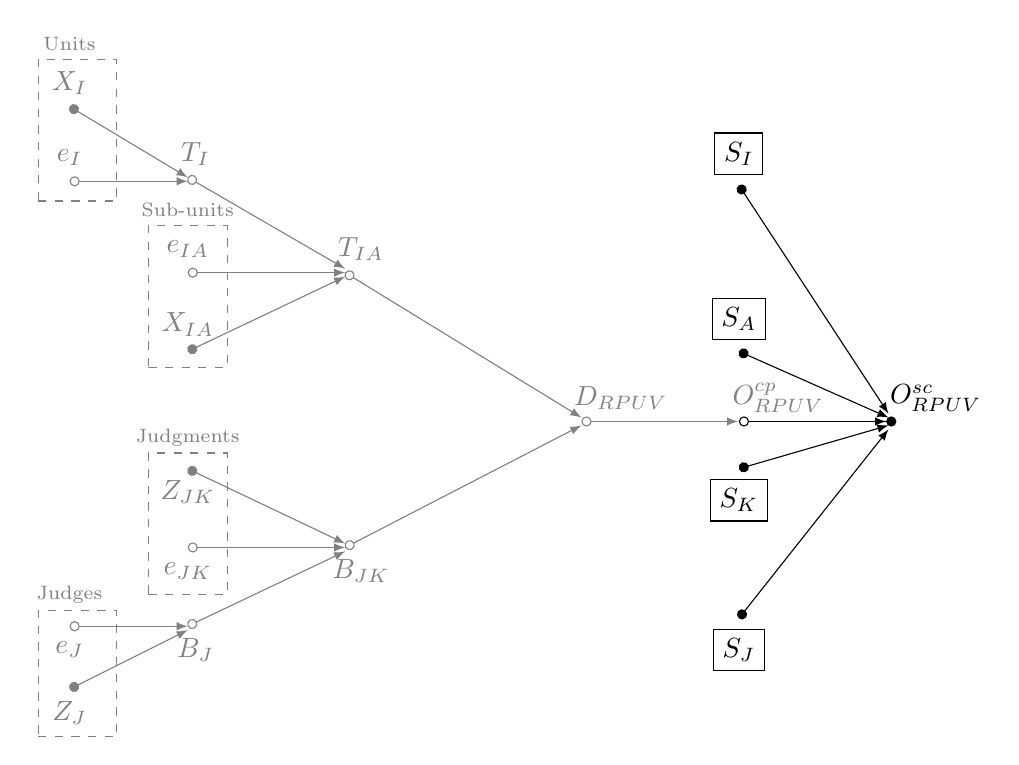
\begin{tikzpicture}

    %%%%%%%%%%%%%%%%%%%%%%%%%%%%%%%%%%%%%%%%%%%%%%%%%%%%%%
    
    % "true" discriminal process for sub-unit
    \node[gray,gray] at (-3.8,1.89) {$T_{IA}$}; %[gray]
    \draw[{Circle[open]}-{latex},gray](-4,1.59) to (-1,-0.25); %,gray

    %%%%%%%%%%%%%%%%%%%%%%%%%%%%%%%%%%%%%%%%%%%%%%%%%%%%%%

    % "true" judgments' bias k_{j}
    \node[gray,gray] at (-3.8,-2.2) {$B_{JK}$}; %[gray]
    \draw[{Circle[open]}-{latex},gray](-4,-1.9) to (-1,-0.35); %,gray

    %%%%%%%%%%%%%%%%%%%%%%%%%%%%%%%%%%%%%%%%%%%%%%%%%%%%%%

    % discriminal difference
    \node[gray,gray] at (-0.5,0) {$D_{RPUV}$}; %[gray]
    %\draw[{Circle[open]}-{latex}{Circle},gray](-1,-0.3) to (1.1,-0.3); %,gray
    
    % complete outcome
    \node[gray,gray] at (1.5,0) {$O^{cp}_{RPUV}$}; %[gray]

    %%%%%%%%%%%%%%%%%%%%%%%%%%%%%%%%%%%%%%%%%%%%%%%%%%%%%%

    % "true" discriminal process of unit
    \node[gray,gray] at (-5.9,3.1) {$T_{I}$}; %[gray]
    \draw[{Circle[open]}-{latex},gray](-6,2.8) to (-4,1.64); %,gray
    
    % sub-units' cluster
    \node[font=\scriptsize,gray] at (-6,2.39) {Sub-units}; %,gray
    \draw[dashed,gray] (-6.5,0.39)--(-5.5,0.39)--(-5.5,2.19)--(-6.5,2.19)--(-6.5,0.39); %,gray
    
    % sub-units error
    \node[gray,gray] at (-6,1.89) {$e_{IA}$}; %[gray]
    \draw[{Circle[open]}-{latex},gray](-6,1.59) to (-4,1.59); %,gray
    
    % predictors for sub-unit
    \node[gray,gray] at (-6,0.93) {$X_{IA}$}; %[gray]
    \draw[{Circle}-{latex},gray](-6,0.59) to (-4,1.54); %,gray

    %%%%%%%%%%%%%%%%%%%%%%%%%%%%%%%%%%%%%%%%%%%%%%%%%%%%%%

    % units' cluster
    \node[font=\scriptsize,gray] at (-7.5,4.5) {Units}; %,gray
    \draw[dashed,gray] (-7.9,2.5)--(-6.9,2.5)--(-6.9,4.3)--(-7.9,4.3)--(-7.9,2.5); %,gray
    
    % predictors for units
    \node[gray,gray] at (-7.5,4) {$X_{I}$}; %[gray]
    \draw[{Circle}-{latex},gray](-7.5,3.7) to (-6,2.8); %,gray

    % units trait error
    \node[gray,gray] at (-7.5,3.05) {$e_{I}$}; %[gray]
    \draw[{Circle[open]}-{latex},gray](-7.5,2.75) to (-6,2.75); %,gray

    %%%%%%%%%%%%%%%%%%%%%%%%%%%%%%%%%%%%%%%%%%%%%%%%%%%%%%

    % judges' bias
    \node[gray,gray] at (-5.9,-3.2) {$B_{J}$}; %[gray]
    \draw[{Circle[open]}-{latex},gray](-6,-2.9) to (-4,-1.95); %,gray

    % judgments' cluster
    \node[font=\scriptsize,gray] at (-6,-0.5) {Judgments}; %,gray
    \draw[dashed,gray] (-6.5,-2.5)--(-5.5,-2.5)--(-5.5,-0.7)--(-6.5,-0.7)--(-6.5,-2.5); %,gray
    
    % judgments' bias error 
    \node[gray,gray] at (-6,-2.2) {$e_{JK}$}; %[gray]
    \draw[{Circle[open]}-{latex},gray](-6,-1.9) to (-4,-1.9); %,gray
    
    % predictors for judgments
    \node[gray,gray] at (-6,-1.2) {$Z_{JK}$}; %[gray]
    \draw[{Circle}-{latex},gray](-6,-0.9) to (-4,-1.85); %,gray
    
    %%%%%%%%%%%%%%%%%%%%%%%%%%%%%%%%%%%%%%%%%%%%%%%%%%%%%%

    % judges' cluster
    \node[font=\scriptsize,gray] at (-7.5,-2.5) {Judges}; %,gray
    \draw[dashed,gray] (-7.9,-4.3)--(-6.9,-4.3)--(-6.9,-2.7)--(-7.9,-2.7)--(-7.9,-4.3); %,gray
    
    % predictors for judges' bias
    \node[gray,gray] at (-7.5,-4) {$Z_{J}$}; %[gray]
    \draw[{Circle}-{latex},gray](-7.5,-3.7) to (-6,-2.95); %,gray
    
    % judges' bias error
    \node[gray,gray] at (-7.5,-3.2) {$e_{J}$}; %[gray]
    \draw[{Circle[open]}-{latex},gray](-7.5,-2.9) to (-6,-2.9); %,gray

    %%%%%%%%%%%%%%%%%%%%%%%%%%%%%%%%%%%%%%%%%%%%%%%%%%%%%%

    % units sampling mechanism
    \node[rectangle,draw] at (1,3.1) {$S_{I}$}; %,gray
    \draw[{Circle}-{latex}](1,2.7) to (2.9,-0.2); %,gray
    
    % subunits sampling mechanism
    \node[rectangle,draw] at (1,1) {$S_{A}$}; %,gray
    \draw[{Circle}-{latex}](1,0.59) to (2.9,-0.25); %,gray
    
    % judgments sampling mechanism
    \node[rectangle,draw] at (1,-1.3) {$S_{K}$}; %,gray
    \draw[{Circle}-{latex}](1,-0.9) to (2.9,-0.35); %,gray
    
    % judges sampling mechanism
    \node[rectangle,draw] at (1,-3.2) {$S_{J}$}; %,gray
    \draw[{Circle}-{latex}](1,-2.8) to (2.9,-0.4); %,gray
    
    % sample outcome
    \node at (3.5,0) {$O^{sc}_{RPUV}$}; %[gray]
    \draw[{Circle[open]}-{latex},gray](-1,-0.3) to (0.99,-0.3); %,gray
    \draw[{Circle[open]}-{latex}{Circle}](1,-0.3) to (3,-0.3); %,gray
    %\draw[{Circle[open]}-{latex}](1,-0.3) to (2.9,-0.3); %,gray
    
    %%%%%%%%%%%%%%%%%%%%%%%%%%%%%%%%%%%%%%%%%%%%%%%%%%%%%%

    % comparison mechanism 
    %\node[rectangle,draw] at (3,3.1) {$C$}; %,gray
    %\draw[{Circle}-{latex}](3,2.7) to (4.8,-0.25); %,gray
    
    % observed outcome
    %\node[gray] at (5.4,0) {$O_{RPUV}$}; %[gray]
    %\draw[{Circle[open]}-{latex}{Circle}](2.9,-0.3) to (4.9,-0.3); %,gray
        
\end{tikzpicture}

\end{document}
